
%% This style is provided exclusively for the ICSE 2012 main conference,
%% ICSE 2012 co-located events, and ICSE 2012 workshops.

%% bare_conf_ICSE12.tex
%% V1.4
%% 2012-01-21
%%

%% This is a skeleton file demonstrating the use of IEEEtran.cls
%% (requires IEEEtran.cls version 1.7 or later) with an IEEE conference paper.
%%
%% Support sites:
%% http://www.michaelshell.org/tex/ieeetran/
%% http://www.ctan.org/tex-archive/macros/latex/contrib/IEEEtran/
%% and
%% http://www.ieee.org/

%%*************************************************************************
%% Legal Notice:
%% This code is offered as-is without any warranty either expressed or
%% implied; without even the implied warranty of MERCHANTABILITY or
%% FITNESS FOR A PARTICULAR PURPOSE! 
%% User assumes all risk.
%% In no event shall IEEE or any contributor to this code be liable for
%% any damages or losses, including, but not limited to, incidental,
%% consequential, or any other damages, resulting from the use or misuse
%% of any information contained here.
%%
%% All comments are the opinions of their respective authors and are not
%% necessarily endorsed by the IEEE.
%%
%% This work is distributed under the LaTeX Project Public License (LPPL)
%% ( http://www.latex-project.org/ ) version 1.3, and may be freely used,
%% distributed and modified. A copy of the LPPL, version 1.3, is included
%% in the base LaTeX documentation of all distributions of LaTeX released
%% 2003/12/01 or later.
%% Retain all contribution notices and credits.
%% ** Modified files should be clearly indicated as such, including  **
%% ** renaming them and changing author support contact information. **
%%
%% File list of work: IEEEtran.cls, IEEEtran_HOWTO.pdf, bare_adv.tex,
%%                    bare_conf.tex, bare_jrnl.tex, bare_jrnl_compsoc.tex
%%*************************************************************************

% *** Authors should verify (and, if needed, correct) their LaTeX system  ***
% *** with the testflow diagnostic prior to trusting their LaTeX platform ***
% *** with production work. IEEE's font choices can trigger bugs that do  ***
% *** not appear when using other class files.                            ***
% The testflow support page is at:
% http://www.michaelshell.org/tex/testflow/



% Note that the a4paper option is mainly intended so that authors in
% countries using A4 can easily print to A4 and see how their papers will
% look in print - the typesetting of the document will not typically be
% affected with changes in paper size (but the bottom and side margins will).
% Use the testflow package mentioned above to verify correct handling of
% both paper sizes by the user's LaTeX system.
%
% Also note that the "draftcls" or "draftclsnofoot", not "draft", option
% should be used if it is desired that the figures are to be displayed in
% draft mode.
%
\documentclass[10pt, conference, compsocconf]{IEEEtran}

% Add the compsocconf option for Computer Society conferences.
%
% If IEEEtran.cls has not been installed into the LaTeX system files,
% manually specify the path to it like:
% \documentclass[conference]{../sty/IEEEtran}


\usepackage{balance}
\usepackage{listings}
\usepackage[pdftex]{graphicx}

\newcommand{\codefamily}{\sffamily}
\newcommand{\csharp}{C\#}
\newcommand{\code}[1]{\lstinline[basicstyle=\codefamily\small]{#1}}
\lstset{language={[Sharp]C},mathescape=false,flexiblecolumns=true,morekeywords={alloc,delay,delete,expose,let,unsatisfiable,receive,rep,contract,message,state,one},basicstyle=\codefamily\footnotesize,literate={->}{{$\rightarrow$}}{2}{<<}{{$\langle$}}{2}{>>}{{$\rangle$}}{2}{!}{{\textbf{!}}}{2},frame=lines,moredelim=[is][\itshape]{@}{@},captionpos=b,numberstyle=\tiny,stepnumber=1,numbersep=2pt}


\newcommand{\comment}[1]{}

% Some very useful LaTeX packages include:
% (uncomment the ones you want to load)


% *** MISC UTILITY PACKAGES ***
%
%\usepackage{ifpdf}
% Heiko Oberdiek's ifpdf.sty is very useful if you need conditional
% compilation based on whether the output is pdf or dvi.
% usage:
% \ifpdf
%   % pdf code
% \else
%   % dvi code
% \fi
% The latest version of ifpdf.sty can be obtained from:
% http://www.ctan.org/tex-archive/macros/latex/contrib/oberdiek/
% Also, note that IEEEtran.cls V1.7 and later provides a builtin
% \ifCLASSINFOpdf conditional that works the same way.
% When switching from latex to pdflatex and vice-versa, the compiler may
% have to be run twice to clear warning/error messages.






% *** CITATION PACKAGES ***
%
%\usepackage{cite}
% cite.sty was written by Donald Arseneau
% V1.6 and later of IEEEtran pre-defines the format of the cite.sty package
% \cite{} output to follow that of IEEE. Loading the cite package will
% result in citation numbers being automatically sorted and properly
% "compressed/ranged". e.g., [1], [9], [2], [7], [5], [6] without using
% cite.sty will become [1], [2], [5]--[7], [9] using cite.sty. cite.sty's
% \cite will automatically add leading space, if needed. Use cite.sty's
% noadjust option (cite.sty V3.8 and later) if you want to turn this off.
% cite.sty is already installed on most LaTeX systems. Be sure and use
% version 4.0 (2003-05-27) and later if using hyperref.sty. cite.sty does
% not currently provide for hyperlinked citations.
% The latest version can be obtained at:
% http://www.ctan.org/tex-archive/macros/latex/contrib/cite/
% The documentation is contained in the cite.sty file itself.






% *** GRAPHICS RELATED PACKAGES ***
%
\ifCLASSINFOpdf
  % \usepackage[pdftex]{graphicx}
  % declare the path(s) where your graphic files are
  % \graphicspath{{../pdf/}{../jpeg/}}
  % and their extensions so you won't have to specify these with
  % every instance of \includegraphics
  % \DeclareGraphicsExtensions{.pdf,.jpeg,.png}
\else
  % or other class option (dvipsone, dvipdf, if not using dvips). graphicx
  % will default to the driver specified in the system graphics.cfg if no
  % driver is specified.
  % \usepackage[dvips]{graphicx}
  % declare the path(s) where your graphic files are
  % \graphicspath{{../eps/}}
  % and their extensions so you won't have to specify these with
  % every instance of \includegraphics
  % \DeclareGraphicsExtensions{.eps}
\fi
% graphicx was written by David Carlisle and Sebastian Rahtz. It is
% required if you want graphics, photos, etc. graphicx.sty is already
% installed on most LaTeX systems. The latest version and documentation can
% be obtained at: 
% http://www.ctan.org/tex-archive/macros/latex/required/graphics/
% Another good source of documentation is "Using Imported Graphics in
% LaTeX2e" by Keith Reckdahl which can be found as epslatex.ps or
% epslatex.pdf at: http://www.ctan.org/tex-archive/info/
%
% latex, and pdflatex in dvi mode, support graphics in encapsulated
% postscript (.eps) format. pdflatex in pdf mode supports graphics
% in .pdf, .jpeg, .png and .mps (metapost) formats. Users should ensure
% that all non-photo figures use a vector format (.eps, .pdf, .mps) and
% not a bitmapped formats (.jpeg, .png). IEEE frowns on bitmapped formats
% which can result in "jaggedy"/blurry rendering of lines and letters as
% well as large increases in file sizes.
%
% You can find documentation about the pdfTeX application at:
% http://www.tug.org/applications/pdftex





% *** MATH PACKAGES ***
%
%\usepackage[cmex10]{amsmath}
% A popular package from the American Mathematical Society that provides
% many useful and powerful commands for dealing with mathematics. If using
% it, be sure to load this package with the cmex10 option to ensure that
% only type 1 fonts will utilized at all point sizes. Without this option,
% it is possible that some math symbols, particularly those within
% footnotes, will be rendered in bitmap form which will result in a
% document that can not be IEEE Xplore compliant!
%
% Also, note that the amsmath package sets \interdisplaylinepenalty to 10000
% thus preventing page breaks from occurring within multiline equations. Use:
%\interdisplaylinepenalty=2500
% after loading amsmath to restore such page breaks as IEEEtran.cls normally
% does. amsmath.sty is already installed on most LaTeX systems. The latest
% version and documentation can be obtained at:
% http://www.ctan.org/tex-archive/macros/latex/required/amslatex/math/





% *** SPECIALIZED LIST PACKAGES ***
%
%\usepackage{algorithmic}
% algorithmic.sty was written by Peter Williams and Rogerio Brito.
% This package provides an algorithmic environment fo describing algorithms.
% You can use the algorithmic environment in-text or within a figure
% environment to provide for a floating algorithm. Do NOT use the algorithm
% floating environment provided by algorithm.sty (by the same authors) or
% algorithm2e.sty (by Christophe Fiorio) as IEEE does not use dedicated
% algorithm float types and packages that provide these will not provide
% correct IEEE style captions. The latest version and documentation of
% algorithmic.sty can be obtained at:
% http://www.ctan.org/tex-archive/macros/latex/contrib/algorithms/
% There is also a support site at:
% http://algorithms.berlios.de/index.html
% Also of interest may be the (relatively newer and more customizable)
% algorithmicx.sty package by Szasz Janos:
% http://www.ctan.org/tex-archive/macros/latex/contrib/algorithmicx/




% *** ALIGNMENT PACKAGES ***
%
%\usepackage{array}
% Frank Mittelbach's and David Carlisle's array.sty patches and improves
% the standard LaTeX2e array and tabular environments to provide better
% appearance and additional user controls. As the default LaTeX2e table
% generation code is lacking to the point of almost being broken with
% respect to the quality of the end results, all users are strongly
% advised to use an enhanced (at the very least that provided by array.sty)
% set of table tools. array.sty is already installed on most systems. The
% latest version and documentation can be obtained at:
% http://www.ctan.org/tex-archive/macros/latex/required/tools/


%\usepackage{mdwmath}
%\usepackage{mdwtab}
% Also highly recommended is Mark Wooding's extremely powerful MDW tools,
% especially mdwmath.sty and mdwtab.sty which are used to format equations
% and tables, respectively. The MDWtools set is already installed on most
% LaTeX systems. The lastest version and documentation is available at:
% http://www.ctan.org/tex-archive/macros/latex/contrib/mdwtools/


% IEEEtran contains the IEEEeqnarray family of commands that can be used to
% generate multiline equations as well as matrices, tables, etc., of high
% quality.


%\usepackage{eqparbox}
% Also of notable interest is Scott Pakin's eqparbox package for creating
% (automatically sized) equal width boxes - aka "natural width parboxes".
% Available at:
% http://www.ctan.org/tex-archive/macros/latex/contrib/eqparbox/





% *** SUBFIGURE PACKAGES ***
%\usepackage[tight,footnotesize]{subfigure}
% subfigure.sty was written by Steven Douglas Cochran. This package makes it
% easy to put subfigures in your figures. e.g., "Figure 1a and 1b". For IEEE
% work, it is a good idea to load it with the tight package option to reduce
% the amount of white space around the subfigures. subfigure.sty is already
% installed on most LaTeX systems. The latest version and documentation can
% be obtained at:
% http://www.ctan.org/tex-archive/obsolete/macros/latex/contrib/subfigure/
% subfigure.sty has been superceeded by subfig.sty.



%\usepackage[caption=false]{caption}
%\usepackage[font=footnotesize]{subfig}
% subfig.sty, also written by Steven Douglas Cochran, is the modern
% replacement for subfigure.sty. However, subfig.sty requires and
% automatically loads Axel Sommerfeldt's caption.sty which will override
% IEEEtran.cls handling of captions and this will result in nonIEEE style
% figure/table captions. To prevent this problem, be sure and preload
% caption.sty with its "caption=false" package option. This is will preserve
% IEEEtran.cls handing of captions. Version 1.3 (2005/06/28) and later 
% (recommended due to many improvements over 1.2) of subfig.sty supports
% the caption=false option directly:
%\usepackage[caption=false,font=footnotesize]{subfig}
%
% The latest version and documentation can be obtained at:
% http://www.ctan.org/tex-archive/macros/latex/contrib/subfig/
% The latest version and documentation of caption.sty can be obtained at:
% http://www.ctan.org/tex-archive/macros/latex/contrib/caption/




% *** FLOAT PACKAGES ***
%
%\usepackage{fixltx2e}
% fixltx2e, the successor to the earlier fix2col.sty, was written by
% Frank Mittelbach and David Carlisle. This package corrects a few problems
% in the LaTeX2e kernel, the most notable of which is that in current
% LaTeX2e releases, the ordering of single and double column floats is not
% guaranteed to be preserved. Thus, an unpatched LaTeX2e can allow a
% single column figure to be placed prior to an earlier double column
% figure. The latest version and documentation can be found at:
% http://www.ctan.org/tex-archive/macros/latex/base/



%\usepackage{stfloats}
% stfloats.sty was written by Sigitas Tolusis. This package gives LaTeX2e
% the ability to do double column floats at the bottom of the page as well
% as the top. (e.g., "\begin{figure*}[!b]" is not normally possible in
% LaTeX2e). It also provides a command:
%\fnbelowfloat
% to enable the placement of footnotes below bottom floats (the standard
% LaTeX2e kernel puts them above bottom floats). This is an invasive package
% which rewrites many portions of the LaTeX2e float routines. It may not work
% with other packages that modify the LaTeX2e float routines. The latest
% version and documentation can be obtained at:
% http://www.ctan.org/tex-archive/macros/latex/contrib/sttools/
% Documentation is contained in the stfloats.sty comments as well as in the
% presfull.pdf file. Do not use the stfloats baselinefloat ability as IEEE
% does not allow \baselineskip to stretch. Authors submitting work to the
% IEEE should note that IEEE rarely uses double column equations and
% that authors should try to avoid such use. Do not be tempted to use the
% cuted.sty or midfloat.sty packages (also by Sigitas Tolusis) as IEEE does
% not format its papers in such ways.





% *** PDF, URL AND HYPERLINK PACKAGES ***
%
\usepackage{url}
% url.sty was written by Donald Arseneau. It provides better support for
% handling and breaking URLs. url.sty is already installed on most LaTeX
% systems. The latest version can be obtained at:
% http://www.ctan.org/tex-archive/macros/latex/contrib/misc/
% Read the url.sty source comments for usage information. Basically,
% \url{my_url_here}.





% *** Do not adjust lengths that control margins, column widths, etc. ***
% *** Do not use packages that alter fonts (such as pslatex).         ***
% There should be no need to do such things with IEEEtran.cls V1.6 and later.
% (Unless specifically asked to do so by the journal or conference you plan
% to submit to, of course. )


% correct bad hyphenation here
\hyphenation{op-tical net-works semi-conduc-tor}


\begin{document}
%
% paper title
% can use linebreaks \\ within to get better formatting as desired
\title{Integrating a Set of Contract Checking Tools into Visual Studio}


% author names and affiliations
% use a multiple column layout for up to two different
% affiliations

\author{\IEEEauthorblockN{Manuel F\"ahndrich, Michael Barnett, Daan
    Leijen, Francesco Logozzo}
\IEEEauthorblockA{Microsoft Research\\
Redmond, USA}
}

% conference papers do not typically use \thanks and this command
% is locked out in conference mode. If really needed, such as for
% the acknowledgment of grants, issue a \IEEEoverridecommandlockouts
% after \documentclass

% for over three affiliations, or if they all won't fit within the width
% of the page, use this alternative format:
% 
%\author{\IEEEauthorblockN{Michael Shell\IEEEauthorrefmark{1},
%Homer Simpson\IEEEauthorrefmark{2},
%James Kirk\IEEEauthorrefmark{3}, 
%Montgomery Scott\IEEEauthorrefmark{3} and
%Eldon Tyrell\IEEEauthorrefmark{4}}
%\IEEEauthorblockA{\IEEEauthorrefmark{1}School of Electrical and Computer Engineering\\
%Georgia Institute of Technology,
%Atlanta, Georgia 30332--0250\\ Email: see http://www.michaelshell.org/contact.html}
%\IEEEauthorblockA{\IEEEauthorrefmark{2}Twentieth Century Fox, Springfield, USA\\
%Email: homer@thesimpsons.com}
%\IEEEauthorblockA{\IEEEauthorrefmark{3}Starfleet Academy, San Francisco, California 96678-2391\\
%Telephone: (800) 555--1212, Fax: (888) 555--1212}
%\IEEEauthorblockA{\IEEEauthorrefmark{4}Tyrell Inc., 123 Replicant Street, Los Angeles, California 90210--4321}}




% use for special paper notices
%\IEEEspecialpapernotice{(Invited Paper)}




% make the title area
\maketitle


\begin{abstract}
Integrating tools and extensions into existing languages, compilers,
debuggers, and IDEs can be difficult, work-intensive, and often
results in a one-off integration.  In this paper, we report on our
experience of building and integrating the CodeContract tool set into an
existing programming environment. The CodeContract tools enable 1)
authoring of contracts (preconditions, postconditions, and object
invariants), 2) instrumenting contract checks into code, 3) statically
checking code against contracts, and 4) visualizing contracts and
results. We identify three characteristics of our integration that
allowed us to reuse existing compilers and IDEs, increase the reach of our tools
to multiple languages and target platforms, and maintain the tools 
over three consecutive versions of C\# and Visual Studio with little effort.
These principles are 1) use source embedding for new language
features, 2) use target analysis and rewriting, and 3) use generic
plug-ins to isolate tools from the IDE.
\end{abstract}

\begin{IEEEkeywords}
tools; plug-ins; contracts; IDE
\end{IEEEkeywords}


% For peer review papers, you can put extra information on the cover
% page as needed:
% \ifCLASSOPTIONpeerreview
% \begin{center} \bfseries EDICS Category: 3-BBND \end{center}
% \fi
%
% For peerreview papers, this IEEEtran command inserts a page break and
% creates the second title. It will be ignored for other modes.
\IEEEpeerreviewmaketitle



\section{Introduction}
% no \IEEEPARstart
\noindent
Programming language researchers and professional tool writers need to
get their language extensions and analysis tools into the hands of
professional developers in order to have impact and learn from user
experience. On the other side, the professional programmer requires
tools to provide 1) easy adoption, 2) immediate benefit, and 3) low
risk.

Teams consist of many developers with established development,
build, and test practices. \emph{Easy adoption} of a tool means that these
practices are impacted minimally. This requirement leaves tool writers with little
space in which to deviate from existing practice. 
In particular, developers typically don't have the luxury to switch
languages or programming environments in order to adopt a new
tool. 

Developers need to see \emph{immediate benefit} from using a new tool,
otherwise, it easily falls by the wayside. It may be beneficial
to provide a combination of tools that provide some small immediate
low cost benefit, with the promise of higher long-term benefit at a
higher cost.

Tool writers must attempt to provide \emph{low risk} to teams adopting
the tools. Tools often are buggy; what is the risk of abandoning the tools
when a dead-end is reached? Will it be necessary to change a lot of code or
practice, leading to further cost and delays? If the tools do code
generation, what's the risk of generating bad code that will only
be found after shipping? How easy is it to mitigate this issue?


In this paper, we report on our experience of building and integrating
the CodeContract tools~\cite{codecontracts} into an existing programming
environment. We discuss how we achieved the above mentioned goals of
easy adoption, immediate benefit, and low risk, and how these affected
our design and the integration with the host programming environment,
in our case, Visual Studio.

The main lessons we draw from our experience for integrating into an
existing development environment are:

\textbf{Source Embedding}: Embed new language features into an existing source
  language using only existing language features such as attributes
  and calls to special libraries, rather than new syntax or stylized
  comments.

\textbf{Target Rewriting}: Give semantics to the new features by
  rewriting the compiler output (the target language), rather than the
  source input. Similarly, perform analysis of code at the target
  language level, rather than the source level.

\textbf{Generic Plug-ins}: For IDE integration, write 
  plug-ins that are reusable across many tools rather than a single
  specific one. This means that generic plug-ins are themselves
  pluggable with tool specific extensions. The main two generic
  plug-ins we wrote are 1) a property and settings manager to
  visualize, edit, and persist tool specific settings into whatever
  format the development environment uses to store such info about a
  build unit, and 2) a feedback manager that translates tool output
  such as warnings and errors into IDE specific warning lists and
  source squigglies.

These design decisions have served us well and have provided our tools
with a great amount of \emph{leverage}:
\begin{itemize}
\item The source embedding allows using our language features in both
  \csharp{} and VisualBasic without a single line of change to the
  existing compilers and IDE.
\item Our new features always work with the latest
  version of these languages. During the lifetime of CodeContracts,
  the compilers and languages have changed twice already (v3.5, v4.0, v4.5).
\item Analyzing and rewriting the target instead of the source makes our tools language
  agnostic. The same tools work on \csharp{} and VisualBasic output.
\item The use of generic plug-ins isolates our extensions from changes
  in the underlying IDE. We are on our third version of Visual Studio
  (2008, 2010, and now 2012) with no change to the tools and a few
  minor changes to the installers.
\item The loose integration of our tools at the level of the source language and
  the .NET target language make our tools usable for a variety of
  platforms supported by Visual Studio, namely desktop (VB and C\#),
  Silverlight inside and outside of browser (VB and C\#), Windows
  Phone Applications (VB and C\#), and server
  side ASP.NET and Azure code (VB and C\#).
\end{itemize}
The rest of the paper is organized as follows:
Section~\ref{sec:contracts} provides some background on the contract
tools, Section~\ref{sec:embed} discusses the principles of embedding
and target rewriting we employed, Section~\ref{sec:vs} explains the
MSBuild process and the hooks in Visual Studio necessary for our
approach. Section~\ref{sec:plugins} discusses our generic plug-ins that
isolate our tools from the Visual Studio IDE and Section~\ref{sec:lessons}
recaps our lessons learned.

\section{CodeContracts}
\label{sec:contracts}
\noindent
We use the CodeContracts tools~\cite{embedded-cc-sac-oops-2010,cccheck} as the poster child to illustrate our
preferred methodology for language extension and tool integration.
CodeContracts enable 1) authoring of contracts (preconditions, postconditions, and
object invariants), 2) instrumenting contract checks into code, 3) 
statically checking code against contracts, and 4) visualizing contracts
and results. Upon embarking on this project, we gave
ourselves a firm constraint that the entire tool chain and experience
must integrate into an existing programming environment, in our case,
Visual Studio, benefiting developers who do not have the luxury to
rely on research compilers. We carefully picked our extension and interaction
points in order to 1) minimize the integration work, 2) make our tools
 usable on multiple languages and target platforms, and 3) keep the
 tools working from one version of Visual Studio to the next.

An example of CodeContracts and its embedding in \csharp{} is shown in
Fig.~\ref{fig:example}. The example illustrates the source embedding
approach. We created a library called
\code{Microsoft.Contracts.dll} which contains a class  \code{Contract}
with a number of static methods:  \code{Requires},
\code{Ensures}, etc. These methods return nothing and take a single
boolean argument. In this example, we use calls to these methods to
``declare'' preconditions and postconditions. The C\# compiler 
treats them as ordinary method calls: it typechecks the arguments
and emits MSIL~\cite{MSIL}, an object oriented
bytecode, which evaluates the arguments and  calls the methods.
Such code is not useful to run directly, but our
tools extract the MSIL that evaluates the expressions and the calls
from the target and use them to perform instrumentation, documentation
generation, or static analysis.

It is worth noting that the use of a library does not preclude
later making the special classes and methods of an embedding approach
a more integrated feature. For example, in version v4.0 of the .NET Common Language
Runtime (CLR), the \code{Contract} class and methods were integrated
into the basic class library. Thus, starting with v4.0, the 
external library was no longer necessary. The  library can still be used however
to build for an older version of the CLR, as our tools do not require
the special classes to be in a particular library.

\begin{figure}[bt]
\vspace*{1mm}
\begin{center}
\begin{lstlisting}
string Compute(string str, int index, Collection c, out int len)
{
  Contract.Requires(str == null ||
                      0 <= index && index < str.Length);
  Contract.Ensures(str == null ||
                     !String.IsNullOrEmpty(Contract.Result())
                     && c.Count > Contract.OldValue(c.Count));
  Contract.Ensures(Contract.ValueAtReturn(out len) >= 0 );
  Contract.Ensures(str == null ||
                     Contract.ForAll(
                       0, Contract.ValueAtReturn(out len),
                       i => Contract.Result()[i] == s[i]) );
  ...
}
\end{lstlisting}
\end{center}
\vspace*{-5mm}
\caption{Example of an embedded language feature: CodeContracts}
\label{fig:example}
\vspace*{-3mm}
\end{figure}


\section{Embedding and Target Rewriting}
\label{sec:embed}
\noindent
Programming language extensions have used two main approaches in
the past: 1) entirely new programming languages or syntactic
extensions of existing ones, or 2) stylized comments in existing languages.
  In either case, these approaches
require entire compiler infrastructures to support tools acting on the
new language features. Specialized languages are difficult to get into
general usage, as the compilers and support tools are usually not on
par with commercial product quality. Often such infrastructures need
to track the evolution of some original language (e.g., Spec\#~\cite{SpecSharp} vs. \csharp{} and
JML~\cite{JML} vs. Java), which means they either don't support the same
language, or lag several years behind the features of the main
language.  

To side-step all these issues, we advocate language extensions
via an \emph{embedding}~\cite{embedded-cc-sac-oops-2010} approach.  The idea of embedding a
new feature in an existing programming language is to:
\begin{enumerate}
\item express the new feature as statements in the
  existing language itself consisting of calls to a special library,
\item leverage the existing language
compiler to perform name and overloading resolution, type checking,
and code generation, and to
\item extract the use of the new language feature from the compiled
  target code using decompilation to find the calls (and arguments) to the special library.
\end{enumerate}

The embedded approach for new language features provides
numerous benefits to the programmer:
\begin{itemize}
\item Not only can the existing editor and IDE be used to author the
  new features, but the IDE actively supports writing proper 
  expressions by providing highlighting, completion, intellisense, and
  early feedback on erroneous expressions (due to the fact that the
  existing language will background check the expressions as normal
  code).
\item Refactoring tools work properly on the new features as well, e.g.,
  renaming a parameter will rename any parameter use inside
  a new feature as well. Contrast this to having new features
  implemented via attributes or special comments in code.
\end{itemize}

\noindent Thus, developers don't have to learn a new language, a new compiler,
or a new IDE. Embedding is also beneficial to writers of tools:
\begin{itemize}
  \item Since the features are compiled by the existing
    compiler, the tool writer has no need to duplicate the full
    compiler infrastructure, such as the parser, type
    checker, name and overloading resolution, etc., nor extend the IDE
    to recognize the new constructs.

  \item Extracting the new feature use from the compiled target code as
    opposed to the source code allows the tool writer to deal with a
    smaller and usually better specified language than the original
    source language. In our example, consider the difference in
    complexity between the full \csharp{} language and the relative
    simplicity of the target MSIL intermediate language of
    .NET. Additionally the new features may work on other
    languages that compile to the same target (in our case VisualBasic).
    
  \item The tool writer can typically reuse existing well tested
    infrastructure to manipulate/analyze the target code, such as .NET
    binary reader/writers, or similarly Java byte code
    infrastructures.
\end{itemize}



\subsection*{Risk Mitigation}
\label{sec:mitigation}
In the introduction, we alluded to the need to minimize risk for
adopters of new tools. In particular, it should be possible for
adopters to stop using the tools without negative impact to the
project (beyond the lack of the benefit of the tool itself). In
particular, this implies that dropping the tools should not require any
code changes. 

With source embedding of new features it is thus a good idea to employ
techniques provided by the compiler or pre-processor to make sure that
all new feature use can be \emph{erased} by the compiler via suitable
compiler options. In our example of CodeContracts, we use
\emph{conditional attributes} on our static
methods\footnote{Conditional attributes are a standard \csharp{} and
  VisualBasic feature.}. These attributes
act as an implicit \code{#ifdef CONTRACTS ... #endif} bracketing
around every \emph{use} of our contract methods. As a result, if the
\code{CONTRACTS} symbol is not defined during a build, the code
compiles as if all extension usage had been syntactically erased. This
principle of erasure gives adopting teams a lot of confidence in
trying out new features and tools, since they know they can flip the
switch at any time without negative impact.

The same principle also allows teams to use new features and tools for
debugging only, but ship code that contains no use of new features and
requires no target rewriting. Removing new tools from the critical
path from source to binaries mitigates risk and puts
adopters at ease.


\section{Visual Studio and MSBuild}
\label{sec:vs}
\begin{figure}[tb!]
\begin{center}
  \hspace*{-3mm}\includegraphics[width=1.05\columnwidth]{arch.png}
\end{center}
\caption{Architecture}
\label{fig:arch}
\vspace*{-5mm}
\end{figure}
\noindent
Visual Studio is a full-fledged integrated development environment from
Microsoft. It supports various source languages and target platforms,
has language specific editors with high-lighting and intellisense, and
all the usual bells and whistles one expects from a modern IDE today.

For \csharp{} and VisualBasic, code is grouped into \emph{projects},
where each project consists of a number of source files and results in
a single \emph{managed assembly} containing the metadata and IL
code. These assemblies typically reside in \code{.dll} or \code{.exe}
files. Debugging information for assemblies is stored in separate
\code{.pdb} files.

Project information is stored in project files (\code{.csproj} for
\csharp{} and \code{.vbproj} for VisualBasic). These files 
contain XML conforming to MSBuild~\cite{MSBuild} descriptions. MSBuild
descriptions are similar to the classic Unix Makefiles, and the
\code{msbuild} command corresponds to the classic \code{make} command~\cite{make}.
Project files define source files, build flavor, references to
libraries, target names etc. as \emph{properties}. The project files
don't contain any actual build rules. Build rules are factored
separately in shared files such as \code{CSharp.targets}, \code{VisualBasic.targets}, and \code{Common.targets} which
are included from every project file. These files also contain XML
conforming to MSBuild descriptions. In this case, they contain
definitions of build steps that are parameterized by properties
defined in the project files.
Fig.~\ref{fig:arch} illustrates this situation for a \csharp{} project
called \code{X}. The project file \code{X.csproj} is used by MSBuild to create
\code{X.dll} from the sources using the \csharp{} compiler
\code{csc}. The project file imports the general \csharp{} build rules
via \code{CSharp.targets}, which in turn include general build rules
(for both VisualBasic and \csharp{}) from \code{Common.targets}.

MSBuild is used to build project outputs from the command line as well
as invoked by Visual Studio when a build is triggered via the
IDE. Visual Studio provides a graphical user interface that exposes
the standard project properties of project files. Therefore,
the way Visual Studio controls the build works entirely by it changing
the properties in the project files and letting MSBuild do the build
based on these properties alone.

\subsection*{Hooks}

To influence the build process, the \code{Common.targets} provides a
general hook to import additional MSBuild files. The hook imports all
MSBuild files located in a particular configuration directory on disk.
The \code{Common.targets} build rules are written in such a way as to make
it easy to write additional rules that trigger during a build prior or
after certain other build steps. Therefore, extending and modifying the
standard build requires no changes to any existing build
files. Instead, one simply authors an additional MSBuild description containing new rules
and settings and imports it using the existing build hook. 

Figure~\ref{fig:arch} shows how this hook is used to import the
\code{Contracts.targets} file. It defines how to rewrite project
outputs to instrument contracts or to run the static analysis.
In our example, it adds an extra build step after the
compilation via the \csharp{} compiler \code{csc} to invoke the
contract rewriter \code{ccrewrite} to instrument checks into the
target IL of \code{X.dll}.

The approach of using the existing build hook provided for all project
types makes our approach independent of project type and addresses
some of our overall goals as follows: the alternative approach (no
common build hook) would be to define
a new kind of project type (\csharp{} with contracts, and similarly
for VB and other flavors) and create new
  projects based on this type. The new project type can have its own
  build rules and would not require an existing hook. However, it
  would a) fail the easy adoption test, since developers would not be
  able to use the tools on \emph{existing} projects, b) entail higher risk, as a
  development team would have to change all their projects to switch
  back to not using the tools. With our advocated approach, it is even
  possible for some team members of a development team to use the
  tools, and for other to not install them. The build works in both
  scenarios, one with tools, the other without.

\section{Plug-in Architecture}
\label{sec:plugins}
\noindent
With the build hook described in the previous section, we can
already influence the build in order to run extra tools. In principle, we
don't need any additional integration into the IDE. E.g., to perform
the contract instrumentation step, the project files simply
need to set the property \code{<CCRewrite>} to true and the build
files handle the rest. Similarly, output from the tools such as
warnings are already printed as part of the build log.

Additional integration into the IDE is really only needed to make the tools
more accessible. Normally, developers don't edit the XML in project 
files by hand, nor do they look at the msbuild output log to see
errors. Instead, the IDE provides a graphical user interface to read
and change project settings and synchronizes them with the corresponding properties in the
project files. Similarly, the IDE takes care of
nicely displaying warnings and errors in a sortable list, and
additionally may overlay squigglies or context menus over the source code.

Thus, in order to make our tools more accessible, we wrote two generic
plug-ins for Visual Studio that we describe in the next sections.

\begin{figure*}[tb!]
\begin{center}
  \hspace*{-3mm}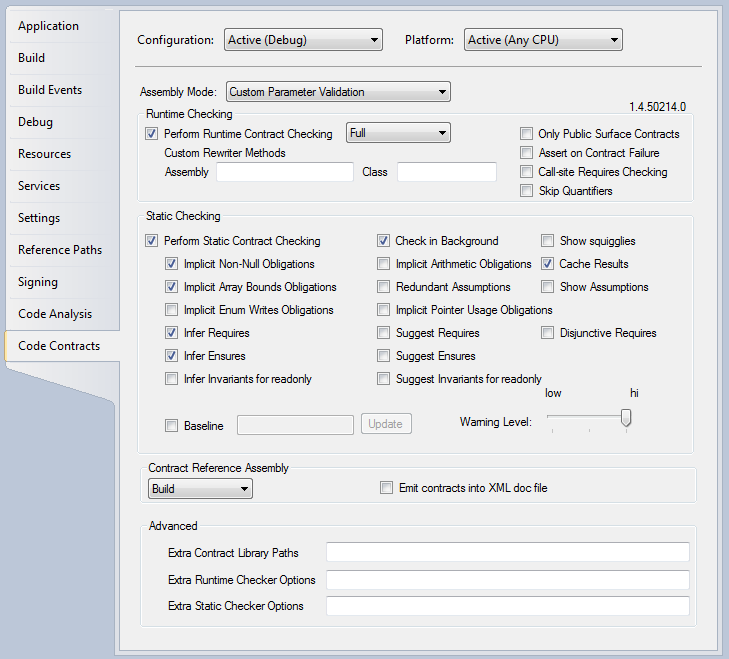
\includegraphics[width=1.3\columnwidth]{propertyUI.png}
\end{center}
\vspace*{-3mm}
\caption{CodeContract Property User Interface}
\label{fig:propertyui}
\vspace*{-3mm}
\end{figure*}

\subsection{Property Manager}
The property manager is a generic plug-in written as a Visual Studio
package. It provides an interface for additional plug-ins to read and
write tool specific project properties into existing project files of
\csharp{} and VisualBasic. Specific plug-ins into the
property manager consist of a UI component typically showing check
marks and other setting elements. In our example, the contract
settings plug-in shown in Figure~\ref{fig:arch} on the top-right plugs
into the generic property manager to read contract specific settings
from the project file, display them, and to write changes from user
manipulations back to the project file via the property manager.

The property manager provides an important level of isolation and
abstraction from the underlying IDE. Implementing the property manager
was quite difficult. To properly interface with Visual Studio and
display settings on existing project types (such as \csharp{} or
VisualBasic) required a rather deep integration, which is beyond the
casual plug-in writer. The property manager thus encapsulates this
complexity and makes it possible to write many tool specific settings
plug-ins in a very easy way, well within the reach of anyone who can
write some simple \csharp{} or VisualBasic code. Additionally, the
property manager isolates tool specific plug-ins from changes in
the underlying IDE due to new versions. 

Our plugin for CodeContract properties works for both \csharp{} and
VisualBasic. In fact, the same component is used for both.  The CodeContract
properties show up after all standard \csharp{}/VB project properties as shown in Fig.~\ref{fig:propertyui}.

\subsection{Feedback Manager}
The feedback manager is our second generic plug-in written as a Visual Studio
package. It provides additional plug-ins an interface to the error list
maintained by the IDE, to source code overlays (such as squigglies to
underline parts of code with warnings), and context menus on warnings
and squigglies. The feedback manager again is generic in that it takes
care of the complicated integration with Visual Studio once and for
all, and provides a simple interface to plug-ins such as the one we
wrote for CodeContracts. The contract specific feedback plug-in uses
context menus to display related warning locations (such as the
location of the original precondition violated at a call site). 

Additionally, the contract specific plug-in into the feedback manager
allows background execution of the static analysis (to avoid
slowing down the build). The same benefits of abstraction and
isolation discussed for the property manager apply equally to the
feedback manager as well.

\section{Lessons Learned}
\label{sec:lessons}
\noindent
In this section, we reflect on our approach and discuss what worked
and why, and point out where our approach has short-comings.

Source embedding of new features and target rewriting worked really
well for tracking language changes and supporting the new features
with the latest language versions. The main reason for this advantage
is that the target language typically evolves much slower than the
source language. This was the case for .NET vs. \csharp{} and
VisualBasic. E.g., in v4.0, \csharp{} added variance for generics,
dynamic types, named arguments and optional parameters, among other
features, whereas the .NET IL didn't change at all. 

The reason why our build integration works well and is stable is
thanks to a good existing design and extensibility of the common MSBuild rules
in the shared \code{Common.targets}. 

\comment{
It is interesting to see how information is exchanged among the
various parts of the IDE and our tools.

\begin{itemize}
\item Properties in msbuild files
\item .NET compiled assemblies (MSIL)
\item PDB files (program debugging information)
\item normal console text output for warnings
\item The Windows Registry
\end{itemize}
}

The languages supported by our approach are not really dependent on
the languages per se, but more by how they integrate into Visual
Studio and the build, and what target binary language they support.
VisualBasic and \csharp{} are integrated very
similarly into Visual Studio and thus our tools work the same on both. C++ and F\#
on the other hand have enough differences that the integration does
not work. For C++ it is the binary target language that is not .NET
and the build process is completely different. For F\#, the
differences are small and our approach should work barring a few
technical difficulties.

Due to our reuse of minimal custom integration, our tools work for a
surprising variety of .NET platform flavors. There are Silverlight
applications running in the browser, or stand-alone, there are ASP.NET
web sites and Azure services with server side .NET code, and Windows Phone
applications. All these platforms have slight differences in library
support, but they share the same source languages, target language,
and build structure. Our tools work with all of these without
change\footnote{The only platform specific code is in selecting the
  appropriate contract reference assemblies for the platform during
  the build.}.

The integration work we did for CodeContracts can be reused in future
tools as most of our integrations are non-tool specific and use
existing hooks provided by Visual Studio. In fact, we already have
used essentially the same approach for other tools, such as the
concurrent revision rewriter~\cite{Burckhardt:revisions}.

Our approach also has short-comings. Target analysis and rewriting is
at the mercy of the precision of debugging information in \code{.pdb} files. E.g., for
.NET source mappings from target IL to source is based on lines only,
so precise intra-line information is not available when highlighting
an expression with a warning. Target rewriting also has the
disadvantage of obscuring high-level constructs in the source language.
E.g., iterators are compiled away into a number of helper classes and
methods. Some decompilation must be performed in order to extract
contracts from such methods.

Another problem we ran into with the build hooks is that they don't
provide any ordering/scheduling support for multiple rewriters in the
tool chain. This makes it difficult to combine tools that don't
know about each other. 


\section{Related Work}
\label{sec:related}
\noindent
The most comparable effort to the CodeContracts tool set and its IDE
integration are the various tools developed for the Java Modeling
Language JML~\cite{JML}. JML uses a comment-based syntax to augment
Java programs with pre and post conditions, and object invariants.
JML has a long history of tools for runtime checking, static checking,
and documentation generation, starting in 1999. As expounded
in~\cite{openJML}, there are at least five distinct efforts and
versions of similar JML tools~\cite{JMLtools,eclipse-jmlc}. All these tools seem to be based on
modified Java compilers that augment various phases to parse the JML
expressions and either translate them to runtime checks, or to various
static checking back-ends. Some tools have various levels of Eclipse IDE~\cite{Eclipse,Eclipse-book}
support.

The JML approach has some advantages over our source embedding
approach: the syntax for contracts can be more concise due to the
ability to step outside the underlying language expression syntax
(e.g., for referring to the result and old-values). Furthermore, we are
relying on conditional compilation features to force erasure of
contracts on builds where they are not desired, comment-based
approaches obviously do not require such features as comments are
erased automatically.

The amount of effort that went into these numerous open-source and
community maintained tools over the years seems disproportionately
larger than our own efforts, and yet has not resulted in a stable set
of tools that has remained up-to-date with the Java language.
In contrast, our
approach and design has not changed since its beginning in 2007. Our
tools have been completely built and maintained by three project
members and two additional researchers, all on a part time basis. Most
of our work has been spent on the actual tooling, such as the static
checker engine, and the rewriting, and very little effort overall went
into the build and IDE integration and its maintenance.






% You must have at least 2 lines in the paragraph with the drop letter
% (should never be an issue)



% An example of a floating figure using the graphicx package.
% Note that \label must occur AFTER (or within) \caption.
% For figures, \caption should occur after the \includegraphics.
% Note that IEEEtran v1.7 and later has special internal code that
% is designed to preserve the operation of \label within \caption
% even when the captionsoff option is in effect. However, because
% of issues like this, it may be the safest practice to put all your
% \label just after \caption rather than within \caption{}.
%
% Reminder: the "draftcls" or "draftclsnofoot", not "draft", class
% option should be used if it is desired that the figures are to be
% displayed while in draft mode.
%
%\begin{figure}[!t]
%\centering
%\includegraphics[width=2.5in]{myfigure}
% where an .eps filename suffix will be assumed under latex, 
% and a .pdf suffix will be assumed for pdflatex; or what has been declared
% via \DeclareGraphicsExtensions.
%\caption{Simulation Results}
%\label{fig_sim}
%\end{figure}

% Note that IEEE typically puts floats only at the top, even when this
% results in a large percentage of a column being occupied by floats.


% An example of a double column floating figure using two subfigures.
% (The subfig.sty package must be loaded for this to work.)
% The subfigure \label commands are set within each subfloat command, the
% \label for the overall figure must come after \caption.
% \hfil must be used as a separator to get equal spacing.
% The subfigure.sty package works much the same way, except \subfigure is
% used instead of \subfloat.
%
%\begin{figure*}[!t]
%\centerline{\subfloat[Case I]\includegraphics[width=2.5in]{subfigcase1}%
%\label{fig_first_case}}
%\hfil
%\subfloat[Case II]{\includegraphics[width=2.5in]{subfigcase2}%
%\label{fig_second_case}}}
%\caption{Simulation results}
%\label{fig_sim}
%\end{figure*}
%
% Note that often IEEE papers with subfigures do not employ subfigure
% captions (using the optional argument to \subfloat), but instead will
% reference/describe all of them (a), (b), etc., within the main caption.


% An example of a floating table. Note that, for IEEE style tables, the 
% \caption command should come BEFORE the table. Table text will default to
% \footnotesize as IEEE normally uses this smaller font for tables.
% The \label must come after \caption as always.
%
%\begin{table}[!t]
%% increase table row spacing, adjust to taste
%\renewcommand{\arraystretch}{1.3}
% if using array.sty, it might be a good idea to tweak the value of
% \extrarowheight as needed to properly center the text within the cells
%\caption{An Example of a Table}
%\label{table_example}
%\centering
%% Some packages, such as MDW tools, offer better commands for making tables
%% than the plain LaTeX2e tabular which is used here.
%\begin{tabular}{|c||c|}
%\hline
%One & Two\\
%\hline
%Three & Four\\
%\hline
%\end{tabular}
%\end{table}


% Note that IEEE does not put floats in the very first column - or typically
% anywhere on the first page for that matter. Also, in-text middle ("here")
% positioning is not used. Most IEEE journals/conferences use top floats
% exclusively. Note that, LaTeX2e, unlike IEEE journals/conferences, places
% footnotes above bottom floats. This can be corrected via the \fnbelowfloat
% command of the stfloats package.



\section{Conclusion}
\label{sec:conclusion}
\noindent
We identified three characteristics that stand out in our effort to
build and integrate a set of contract checking tools into Visual
Studio. 1) Use source embedding for new language features in order to
reuse existing compilers and source editors as-is, 2) use target
analysis and rewriting to isolate from the evolution of source
languages and to support multiple source languages with a common set
of tools, and 3) use generic plug-ins to isolate tools from the IDE.

Our tools and integration have survived three consecutive versions of
the \csharp{} and VisualBasic languages and compilers, as well as three
versions of Visual Studio with little maintenance effort on our part.

If we were to embark on another language extension project, we would
proceed with the same design.


% conference papers do not normally have an appendix


% use section* for acknowledgement
\section*{Acknowledgment}
The authors would like to thank Herman Venter for his tireless efforts
building the best .NET readers and writers.

% trigger a \newpage just before the given reference
% number - used to balance the columns on the last page
% adjust value as needed - may need to be readjusted if
% the document is modified later
%\IEEEtriggeratref{8}
% The "triggered" command can be changed if desired:
%\IEEEtriggercmd{\enlargethispage{-5in}}

% Better way for balancing the last page:

\balance

% references section

% can use a bibliography generated by BibTeX as a .bbl file
% BibTeX documentation can be easily obtained at:
% http://www.ctan.org/tex-archive/biblio/bibtex/contrib/doc/
% The IEEEtran BibTeX style support page is at:
% http://www.michaelshell.org/tex/ieeetran/bibtex/
\bibliographystyle{IEEEtran}
%\bibliographystyle{plain}
% argument is your BibTeX string definitions and bibliography database(s)
%\bibliography{IEEEabrv,../bib/paper}
%
% <OR> manually copy in the resultant .bbl file
% set second argument of \begin to the number of references
% (used to reserve space for the reference number labels box)

\bibliography{ccvs}

%\begin{thebibliography}{1}

%\bibitem{IEEEhowto:kopka}
%H.~Kopka and P.~W. Daly, \emph{A Guide to \LaTeX}, 3rd~ed.\hskip 1em plus
%  0.5em minus 0.4em\relax Harlow, England: Addison-Wesley, 1999.

%\end{thebibliography}




% that's all folks
\end{document}


